\documentclass[11pt]{article}
\usepackage[letterpaper,margin=0.75in,headheight=14pt]{geometry}
\usepackage{amsmath,amssymb,enumitem,graphicx,booktabs,fancyhdr}
\pagestyle{fancy}\fancyhf{}
\lhead{\small Test Study Guide: 5.7--6.2a}\rhead{\small Calculus BC}\cfoot{\thepage}
\setlength{\parindent}{0pt}
\newcommand{\wsS}{\vspace*{3cm}}
\newcommand{\wsM}{\vspace*{4.5cm}}
\newcommand{\wsL}{\vspace*{6.5cm}}
\newcommand{\wsG}{\vspace*{2cm}}
\newcommand{\prob}[1]{\par\noindent\textbf{#1.}\quad}
\newcommand{\ansitem}[1]{\item[\textbf{#1.}]}
\newcommand{\figurehere}[2]{\par\smallskip\centerline{\includegraphics[height=#2]{fig-test-5.7-6.2a-q#1.png}}\smallskip}
\begin{document}
Name: \rule{2.7in}{0.4pt}\hfill Date: \rule{1.3in}{0.4pt}\par\bigskip

\prob{1} Approximate the definite integral using the trapezoidal rule with $n=6$.
Approximate each function value to four decimal places and round the final answer to two decimal places.
\[\int_1^4\frac{1}{x}\,dx\]
\wsM
\prob{2} Evaluate.
\[\int\frac{1}{\sqrt{x}(1+\sqrt{x})^2}\,dx\]
\wsM
\prob{3} Evaluate.
\[\int_0^{\pi/2}\cos x\sqrt{3+5\sin x}\,dx\]
\wsM
\clearpage

\prob{4} Evaluate.
\[\int \frac{d}{dx}\!\left(\sqrt[5]{x^4+2x^2+1}\right)\,dx\]
\wsM
\prob{5} Solve the differential equation subject to the given conditions.
\[\frac{d^2y}{dx^2}=6x-4,\qquad y(2)=4,\qquad y'(2)=5.\]
\wsM
\prob{6} Let $f(x)=9-x^2$ for $-2\leq x\leq3$, and let $P$ be the regular partition of $[-2,3]$ into five subintervals. Find the Riemann sum $R_P$ if $f$ is evaluated at the midpoint of each subinterval of $P$.
\wsM
\clearpage

\prob{7} Express as one integral.
\[\int_c^e f(x)\,dx+\int_a^b f(x)\,dx-\int_c^b f(x)\,dx-\int_d^d f(x)\,dx\]
\wsL
\vfill
\prob{8} Approximate the definite integral using the trapezoidal rule with $n=5$.
Use function values rounded to four decimal places and round the final answer to two decimal places.
\[\int_0^{10}\sqrt{1+x^4}\,dx\]
\wsL
\clearpage

\prob{9} Set up an integral that can be used to find the area of the region bounded by the three labeled curves.
\figurehere{9}{5.5cm}
\wsM
\vfill
\prob{10} Sketch the region bounded by the graphs of the equations and find its area.
\[y=x^2,\qquad y=4x\]
\wsL
\clearpage

\prob{11} Sketch the region bounded by the graphs of the equations and find its area.
\[y=\frac{1}{x^2},\qquad y=-x^2,\qquad x=1,\qquad x=2\]
\wsL
\vfill
\prob{12} Sketch the region bounded by the graphs of the equations and find its area.
\[y=4+x,\qquad y^2+x=2\]
\wsL
\clearpage

\prob{13} Sketch the region bounded by the graphs of the equations and find its area.
\[y=x\sqrt{4-x^2},\qquad y=0\]
\wsL
\vfill
\prob{14} Set up sums of integrals that can be used to find the area of the region enclosed by the three lines shown, integrating with respect to \textbf{(a)} $x$ and \textbf{(b)} $y$.
\figurehere{14}{5.5cm}
\wsM
\clearpage

\prob{15} Set up integrals, or sums of integrals, that can be used to find the area of the region bounded by the graphs, integrating with respect to \textbf{(a)} $x$ and \textbf{(b)} $y$.
\[y=x+3,\qquad x=-y^2+3\]
\wsL
\vfill
\prob{16} The figure shows a stress--strain diagram. Estimate the $y$-coordinates and approximate the area enclosed by the hysteresis loop using the trapezoidal rule with $n=6$.
\figurehere{16}{5.5cm}
\wsM
\clearpage

\prob{17} Set up an integral that can be used to find the volume of the solid obtained by revolving the shaded region about the indicated axis.
\figurehere{17}{5.5cm}
\wsM
\vfill
\prob{18} Sketch the region $R$ bounded by the graphs of the equations. Find the volume of the solid generated if $R$ is revolved about the $x$-axis.
\[y=\sqrt{x},\qquad x=4,\qquad y=0\]
\wsL
\clearpage

\prob{19} Sketch the region $R$ bounded by the graphs of the equations. Find the volume of the solid generated if $R$ is revolved about the $x$-axis.
\[y=x^2-4x,\qquad y=0\]
\wsM
\prob{20} Sketch the region $R$ bounded by the graphs of the equations. Find the volume of the solid generated if $R$ is revolved about the $x$-axis.
\[y=x^3,\qquad x=-2,\qquad y=0\]
\wsM
\prob{21} Sketch the region $R$ bounded by the graphs of the equations. Find the volume of the solid generated if $R$ is revolved about the $y$-axis.
\[x=4y-y^2,\qquad x=0\]
\wsM
\clearpage

\section*{Tommy's Questions}
\prob{Tommy 1} A function $F$ satisfies
\[F'(x)=x\sqrt{1+x^2}\quad(0\leq x\leq2),\qquad F(0)=2.\]
\begin{enumerate}[label=\textbf{(\alph*)},leftmargin=2em,itemsep=4pt]
\item Find an exact formula for $F(x)$.
\item Find the average value of $F'$ on $[0,2]$.
\item Use the trapezoidal rule with four equal subintervals to approximate $F(2)$. Round to three decimal places.
\item Is the approximation in part (c) greater than or less than the exact value? Justify your answer.
\end{enumerate}
\wsL
\clearpage

\prob{Tommy 2} Let $R$ be the region bounded by
\[y=0,\qquad y=\sqrt{\frac{x^{2026}}{x^{2026}+(1-x)^{2026}}},\qquad x=0,\qquad x=1.\]
Find the exact volume of the solid obtained by revolving $R$ about the $x$-axis.
\wsL
\vfill
\prob{Tommy 3} For each $x\in[0,2]$, let $f(x)$ be the unique nonnegative number satisfying
\[[f(x)]^5+f(x)=x.\]
Find the exact volume of the solid obtained by revolving the region bounded by $y=f(x)$, $y=0$, and $x=2$ about the $x$-axis.
\wsL
\clearpage

\section*{Answer Key}
\begin{description}[leftmargin=2.7em,labelwidth=2em,itemsep=11pt]
\ansitem{1} $1.41$.
\ansitem{2} $\displaystyle -\frac{2}{1+\sqrt{x}}+C$.
\ansitem{3} $\displaystyle \frac{32\sqrt{2}-6\sqrt{3}}{15}$.
\ansitem{4} $\displaystyle \sqrt[5]{x^4+2x^2+1}+C$.
\ansitem{5} $\displaystyle y=x^3-2x^2+x+2$.
\ansitem{6} $\displaystyle R_P=\frac{135}{4}$.
\ansitem{7} $\displaystyle \int_a^e f(x)\,dx$.
\ansitem{8} $341.36$.
\ansitem{9} $\displaystyle \int_1^4\left(6-x-\sqrt{x}\right)\,dx$.
\ansitem{10} $\displaystyle A=\frac{32}{3}$.
\ansitem{11} $\displaystyle A=\frac{17}{6}$.
\ansitem{12} $\displaystyle A=\frac{125}{6}$.
\ansitem{13} $\displaystyle A=\frac{16}{3}$ (both regions together).
\ansitem{14} \textbf{(a)} $\displaystyle \int_0^1(3x-x)\,dx+\int_1^2(4-x-x)\,dx$.\par\smallskip
\textbf{(b)} $\displaystyle \int_0^2\left(y-\frac y3\right)\,dy+\int_2^3\left(4-y-\frac y3\right)\,dy$.
\ansitem{15} \textbf{(a)} $\displaystyle \int_{-6}^{-1}\left(x+3+\sqrt{3-x}\right)\,dx+\int_{-1}^3 2\sqrt{3-x}\,dx$.\par\smallskip
\textbf{(b)} $\displaystyle \int_{-3}^2\left[(3-y^2)-(y-3)\right]\,dy$.
\end{description}
\clearpage

\section*{Answer Key (continued)}
\begin{description}[leftmargin=2.7em,labelwidth=2em,itemsep=15pt]
\ansitem{16} Approximately $4.2$ square coordinate units, using the following estimated readings:
\begin{center}\small
\begin{tabular}{lrrrrrrr}\toprule
$x$ & 0 & 1 & 2 & 3 & 4 & 5 & 6\\\midrule
Upper curve & 0 & 1.5 & 2.0 & 2.5 & 3.0 & 3.6 & 5.0\\
Lower curve & 0 & 1.0 & 1.3 & 1.5 & 2.0 & 2.6 & 5.0\\\bottomrule
\end{tabular}\end{center}
Reasonable graph readings give slightly different answers.
\ansitem{17} $\displaystyle V=\pi\int_0^2(4-y^2)^2\,dy$.
\ansitem{18} $\displaystyle V=8\pi$.
\ansitem{19} $\displaystyle V=\frac{512\pi}{15}$.
\ansitem{20} $\displaystyle V=\frac{128\pi}{7}$.
\ansitem{21} $\displaystyle V=\frac{512\pi}{15}$.
\end{description}
\bigskip
\textbf{Tommy 1.}
\begin{enumerate}[label=\textbf{(\alph*)},leftmargin=2em,itemsep=9pt]
\item With $u=1+x^2$ and $du=2x\,dx$,
\[F(x)=\frac13(1+x^2)^{3/2}+C.\]
Since $F(0)=2$, $C=5/3$. Thus $\boxed{F(x)=\frac{(1+x^2)^{3/2}+5}{3}}$.
\item The average value is
\[\frac12\int_0^2 x\sqrt{1+x^2}\,dx
=\frac12\left[\frac{(1+x^2)^{3/2}}3\right]_0^2
=\boxed{\frac{5\sqrt5-1}{6}}.\]
\item Write $g(x)=F'(x)$. With $\Delta x=1/2$,
\[T_4=\frac14\left[g(0)+2g(1/2)+2g(1)+2g(3/2)+g(2)\right]
\approx3.4567.\]
Therefore $F(2)\approx F(0)+T_4=\boxed{5.457}$.
\item $\displaystyle g''(x)=\frac{x(3+2x^2)}{(1+x^2)^{3/2}}>0$ for $0<x\leq2$.
The graph of $g$ is concave up, so the trapezoids overestimate its integral.
Adding $F(0)$ preserves the inequality: the approximation is \textbf{greater} than the exact value.
\end{enumerate}
\clearpage

\section*{Tommy's Questions: Worked Solutions}
\textbf{Tommy 2.} The disk radius is
\[r(x)=\sqrt{\frac{x^{2026}}{x^{2026}+(1-x)^{2026}}}.\]
Therefore
\[V=\pi\int_0^1 r(x)^2\,dx
=\pi\int_0^1\frac{x^{2026}}{x^{2026}+(1-x)^{2026}}\,dx.\]
Let the last integral be $I$. Substituting $u=1-x$ gives
\[I=\int_0^1\frac{(1-u)^{2026}}{u^{2026}+(1-u)^{2026}}\,du.\]
Adding the two expressions yields $2I=\int_0^1 1\,dx=1$.
Thus $\boxed{V=\pi/2}$.
\bigskip

\textbf{Tommy 3.} The disk formula gives
\[V=\pi\int_0^2[f(x)]^2\,dx.\]
Set $y=f(x)$. The defining equation gives $x=y^5+y$ and
$dx=(5y^4+1)\,dy$. Since $5y^4+1>0$, this substitution is increasing.
At $x=0$, $y=0$; at $x=2$, $y=1$.
\begin{align*}
V&=\pi\int_0^1 y^2(5y^4+1)\,dy\\
 &=\pi\left[\frac57y^7+\frac13y^3\right]_0^1
 =\boxed{\frac{22\pi}{21}}.
\end{align*}
The radius is $f(x)$, not $x$. Changing variables avoids solving the fifth-degree equation.
\clearpage

\section*{Answer Key: Region Sketches}
\begin{center}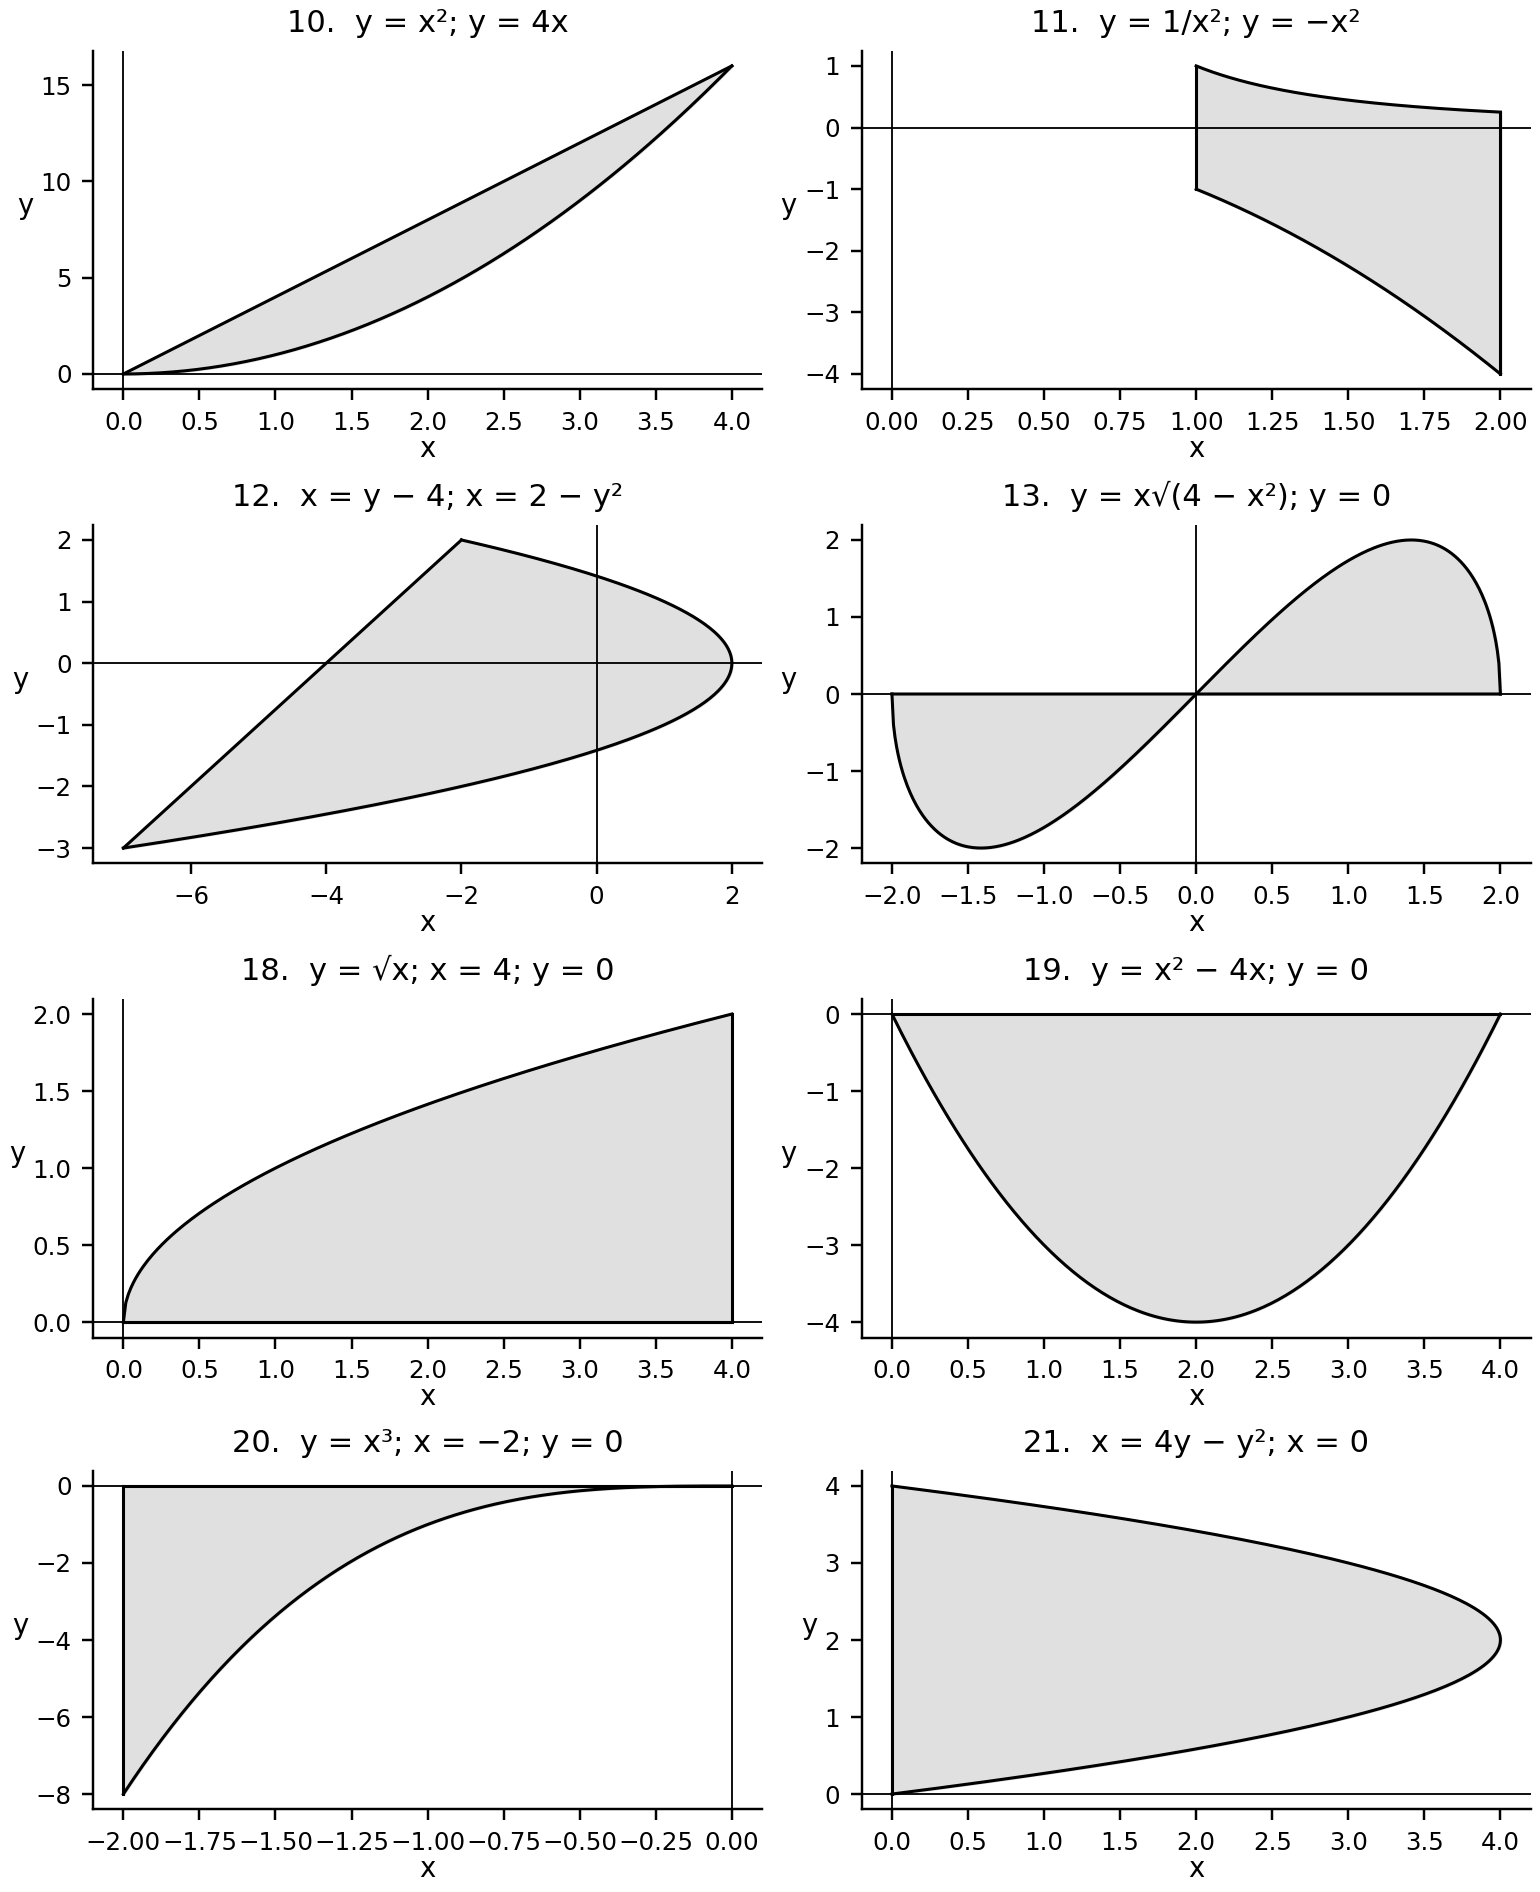
\includegraphics[width=\linewidth,height=8.4in,keepaspectratio]{fig-test-5.7-6.2a-answer-sketches.png}\end{center}
\clearpage

% === SOURCELIST ===
\section*{Where These Questions Came From}
These questions come from Sections 5.7, 5.8, 6.1, and 6.2. Try the surrounding problems for more practice.
\bigskip
\begin{center}
\begin{tabular}{lll}\toprule
Guide question & Section & Exercise\\\midrule
1 & 5.7 & 5(a)\\\midrule
2 & 5.8 & 9\\
3 & 5.8 & 35\\
4 & 5.8 & 39\\
5 & 5.8 & 43\\
6 & 5.8 & 45\\
7 & 5.8 & 49\\
8 & 5.8 & 53(a)\\\midrule
9 & 6.1 & 2\\
10 & 6.1 & 5\\
11 & 6.1 & 9\\
12 & 6.1 & 13\\
13 & 6.1 & 21\\
14 & 6.1 & 25\\
15 & 6.1 & 29\\
16 & 6.1 & 39(a)\\\midrule
17 & 6.2 & 2\\
18 & 6.2 & 6\\
19 & 6.2 & 7\\
20 & 6.2 & 8\\
21 & 6.2 & 11\\\midrule
Tommy 1 & \multicolumn{2}{l}{Original --- not in the textbook}\\
Tommy 2 & \multicolumn{2}{l}{Original --- not in the textbook}\\
Tommy 3 & \multicolumn{2}{l}{Original --- not in the textbook}\\\bottomrule
\end{tabular}
\end{center}
\end{document}
